
%% ══════════════════════════════════════════════════════════════════════════════
%% PART 6: GAMIFIED XR FOR REHABILITATION (5 SLIDES)
%% ══════════════════════════════════════════════════════════════════════════════

\begin{frame}{XR-Based Rehabilitation: Evolution and Current State}
	\textbf{\textcolor{gbAqua}{Historical Trajectory}}
	
	\begin{itemize}
		\item Early 2010s: Conceptual frameworks, proof-of-concept studies
		\item Recent years: Robust systems supporting motor, cognitive, psychosocial interventions
		\item Current status: Increasing feasibility and real-world applicability
	\end{itemize}
	
	\vspace{0.3cm}
	
	\textbf{\textcolor{gbAqua}{Two Complementary Approaches}}
	
	\begin{columns}[t]
		\column{0.48\textwidth}
		\textbf{Standardization}
		
		\begin{itemize}
			\item Uniform, evidence-based protocols
			\item Consistent delivery across patients
			\item Ensures reliability and scalability
		\end{itemize}
		
		\column{0.48\textwidth}
		\textbf{Personalization}
		
		\begin{itemize}
			\item Customization to individual needs
			\item Adaptive parameters (difficulty, feedback, pacing)
			\item Enhanced engagement and outcomes
		\end{itemize}
	\end{columns}
	
	\citefooter{Crowe et al., 2024; Cucinella et al., 2025; Felipe et al., 2020}
\end{frame}

\begin{frame}{Balancing Engagement and Therapeutic Relevance}
	\textbf{\textcolor{gbAqua}{The Central Challenge}}
	
	Pediatric exergames must reconcile two competing demands:
	
	\begin{itemize}
		\item \textbf{Therapeutic specificity}: Movements must be therapeutically meaningful
		\item \textbf{Engagement}: Visual appeal and narrative must sustain motivation
	\end{itemize}
	
	\vspace{0.3cm}
	
	\textbf{\textcolor{gbAqua}{The Design Tension}}
	
	\begin{itemize}
		\item Many research systems prioritize precision over appeal
		\item Result: Limited visual appeal compared to commercial games
		\item Risk: Systems difficult to deploy in clinical/home settings
		\item Commercial games alone (e.g., Wii Sports) → high engagement BUT limited clinical improvement
	\end{itemize}
	
	\vspace{0.3cm}
	
	\textbf{\textcolor{gbAqua}{Solution}}
	
	Dedicated systems that are genuinely enjoyable while ensuring therapeutically meaningful movement repetition
	
	\citefooter{Biffi et al., 2017; Robertson et al., 2010; Chiu et al., 2014}
\end{frame}

\begin{frame}{Exergaming in Pediatric Motor Rehabilitation}
	\textbf{\textcolor{gbAqua}{Clinical Evidence}}
	
	Meta-analysis: VR-assisted exergaming in children with cerebral palsy
	
	\begin{itemize}
		\item 45 studies, 1500+ participants
		\item Significant improvements in global motor function and activities of daily living
		\item Consistently rated as safe and well-accepted
	\end{itemize}
	
	\vspace{0.3cm}
	
	\textbf{\textcolor{gbAqua}{Key Advantages of Well-Designed Exergames}}
	
	\begin{itemize}
		\item Incorporate motor learning principles: repetition, immediate feedback, intrinsic motivation
		\item Multimodal feedback: auditory, visual, haptic cues guide and motivate
		\item Shared play with therapists/caregivers increases engagement and participation
		\item Gamification improves adherence and reduces perceived effort
	\end{itemize}
	
	\citefooter{Tobaiqi et al., 2023; Birckhead et al., 2019}
\end{frame}

\begin{frame}{Personalization vs Standardization in Rehabilitation XR}
	\textbf{\textcolor{gbAqua}{The Heterogeneity Challenge}}
	
	Each child with neuromotor disorder presents:
	\begin{itemize}
		\item Distinct combination of disorder severity
		\item Different physical development stage
		\item Evolving therapeutic needs
	\end{itemize}
	
	\vspace{0.3cm}
	
	\textbf{\textcolor{gbAqua}{Standardization: Foundation}}
	
	\begin{itemize}
		\item Proven safety and usability create infrastructure
		\item Necessary step for wide adoption
		\item May constrain individual adaptation
	\end{itemize}
	
	\vspace{0.3cm}
	
	\textbf{\textcolor{gbAqua}{Personalization: Advanced Stage}}
	
	\begin{itemize}
		\item Customization aligned with specific needs
		\item Requires tools for configuration, monitoring, analysis
		\item Currently uncommon in research studies
		\item Essential for truly effective and meaningful interventions
	\end{itemize}
	
	\citefooter{Felipe et al., 2020; Figueiredo et al., 2025}
\end{frame}

\begin{frame}{Design Principles for Pediatric Exergames}
	\textbf{\textcolor{gbAqua}{Semantic Coherence}}
	
	Movement mapping is intuitive and related to in-game effect
	\begin{itemize}
		\item Rotate wrist to aim (natural mapping)
		\item Lift arm to jump (gravity-respecting)
		\item No memorization of arbitrary mappings required
	\end{itemize}
	
	\vspace{0.2cm}
	
	\textbf{\textcolor{gbAqua}{Accessibility: Multiple Pathways}}
	
	\begin{itemize}
		\item Alternative movement options for diverse abilities
		\item Ensures no child excluded from game aspects
	\end{itemize}
	
	\vspace{0.2cm}
	
	\textbf{\textcolor{gbAqua}{Visual Balance}}
	
	\begin{itemize}
		\item Rich enough to engage (avoid research-app appearance)
		\item Uncluttered enough to focus on task (reduce cognitive overload)
		\item Guided by clinical feedback on pediatric preferences
	\end{itemize}
	
	\vspace{0.2cm}
	
	\textbf{\textcolor{gbAqua}{Multimodal Feedback}}
	
	Visual + Audio + Haptic cues reinforce execution and maintain engagement
\end{frame}

%% ══════════════════════════════════════════════════════════════════════════════
%% PART 7: ACTIVEPAWS SYSTEM (12 SLIDES)
%% ══════════════════════════════════════════════════════════════════════════════

\begin{frame}{The Clinical Challenge: Pediatric Upper Limb Rehabilitation}
	\textbf{\textcolor{gbAqua}{Target Population}}
	
	Children with neuromotor disorders: Cerebral Palsy (CP), Acquired Brain Injury (ABI)
	
	\begin{itemize}
		\item Widely varying residual motor abilities
		\item Limited frustration tolerance
		\item Strong need for intrinsically motivating activities
	\end{itemize}
	
	\vspace{0.3cm}
	
	\textbf{\textcolor{gbAqua}{Why Standard Controllers Don't Work}}
	
	\begin{itemize}
		\item Not designed for children
		\item Require sustained precision gripping
		\item Lack postural support
		\item Poor fine motor affordances for impaired hands
	\end{itemize}
	
	\vspace{0.3cm}
	
	\textbf{\textcolor{gbAqua}{The Wearable Approach}}
	
	Custom orthosis + motion sensing enables postural support, intuitive interaction, and therapeutic movement mapping
\end{frame}

\begin{frame}{ActivePaws System Architecture}
	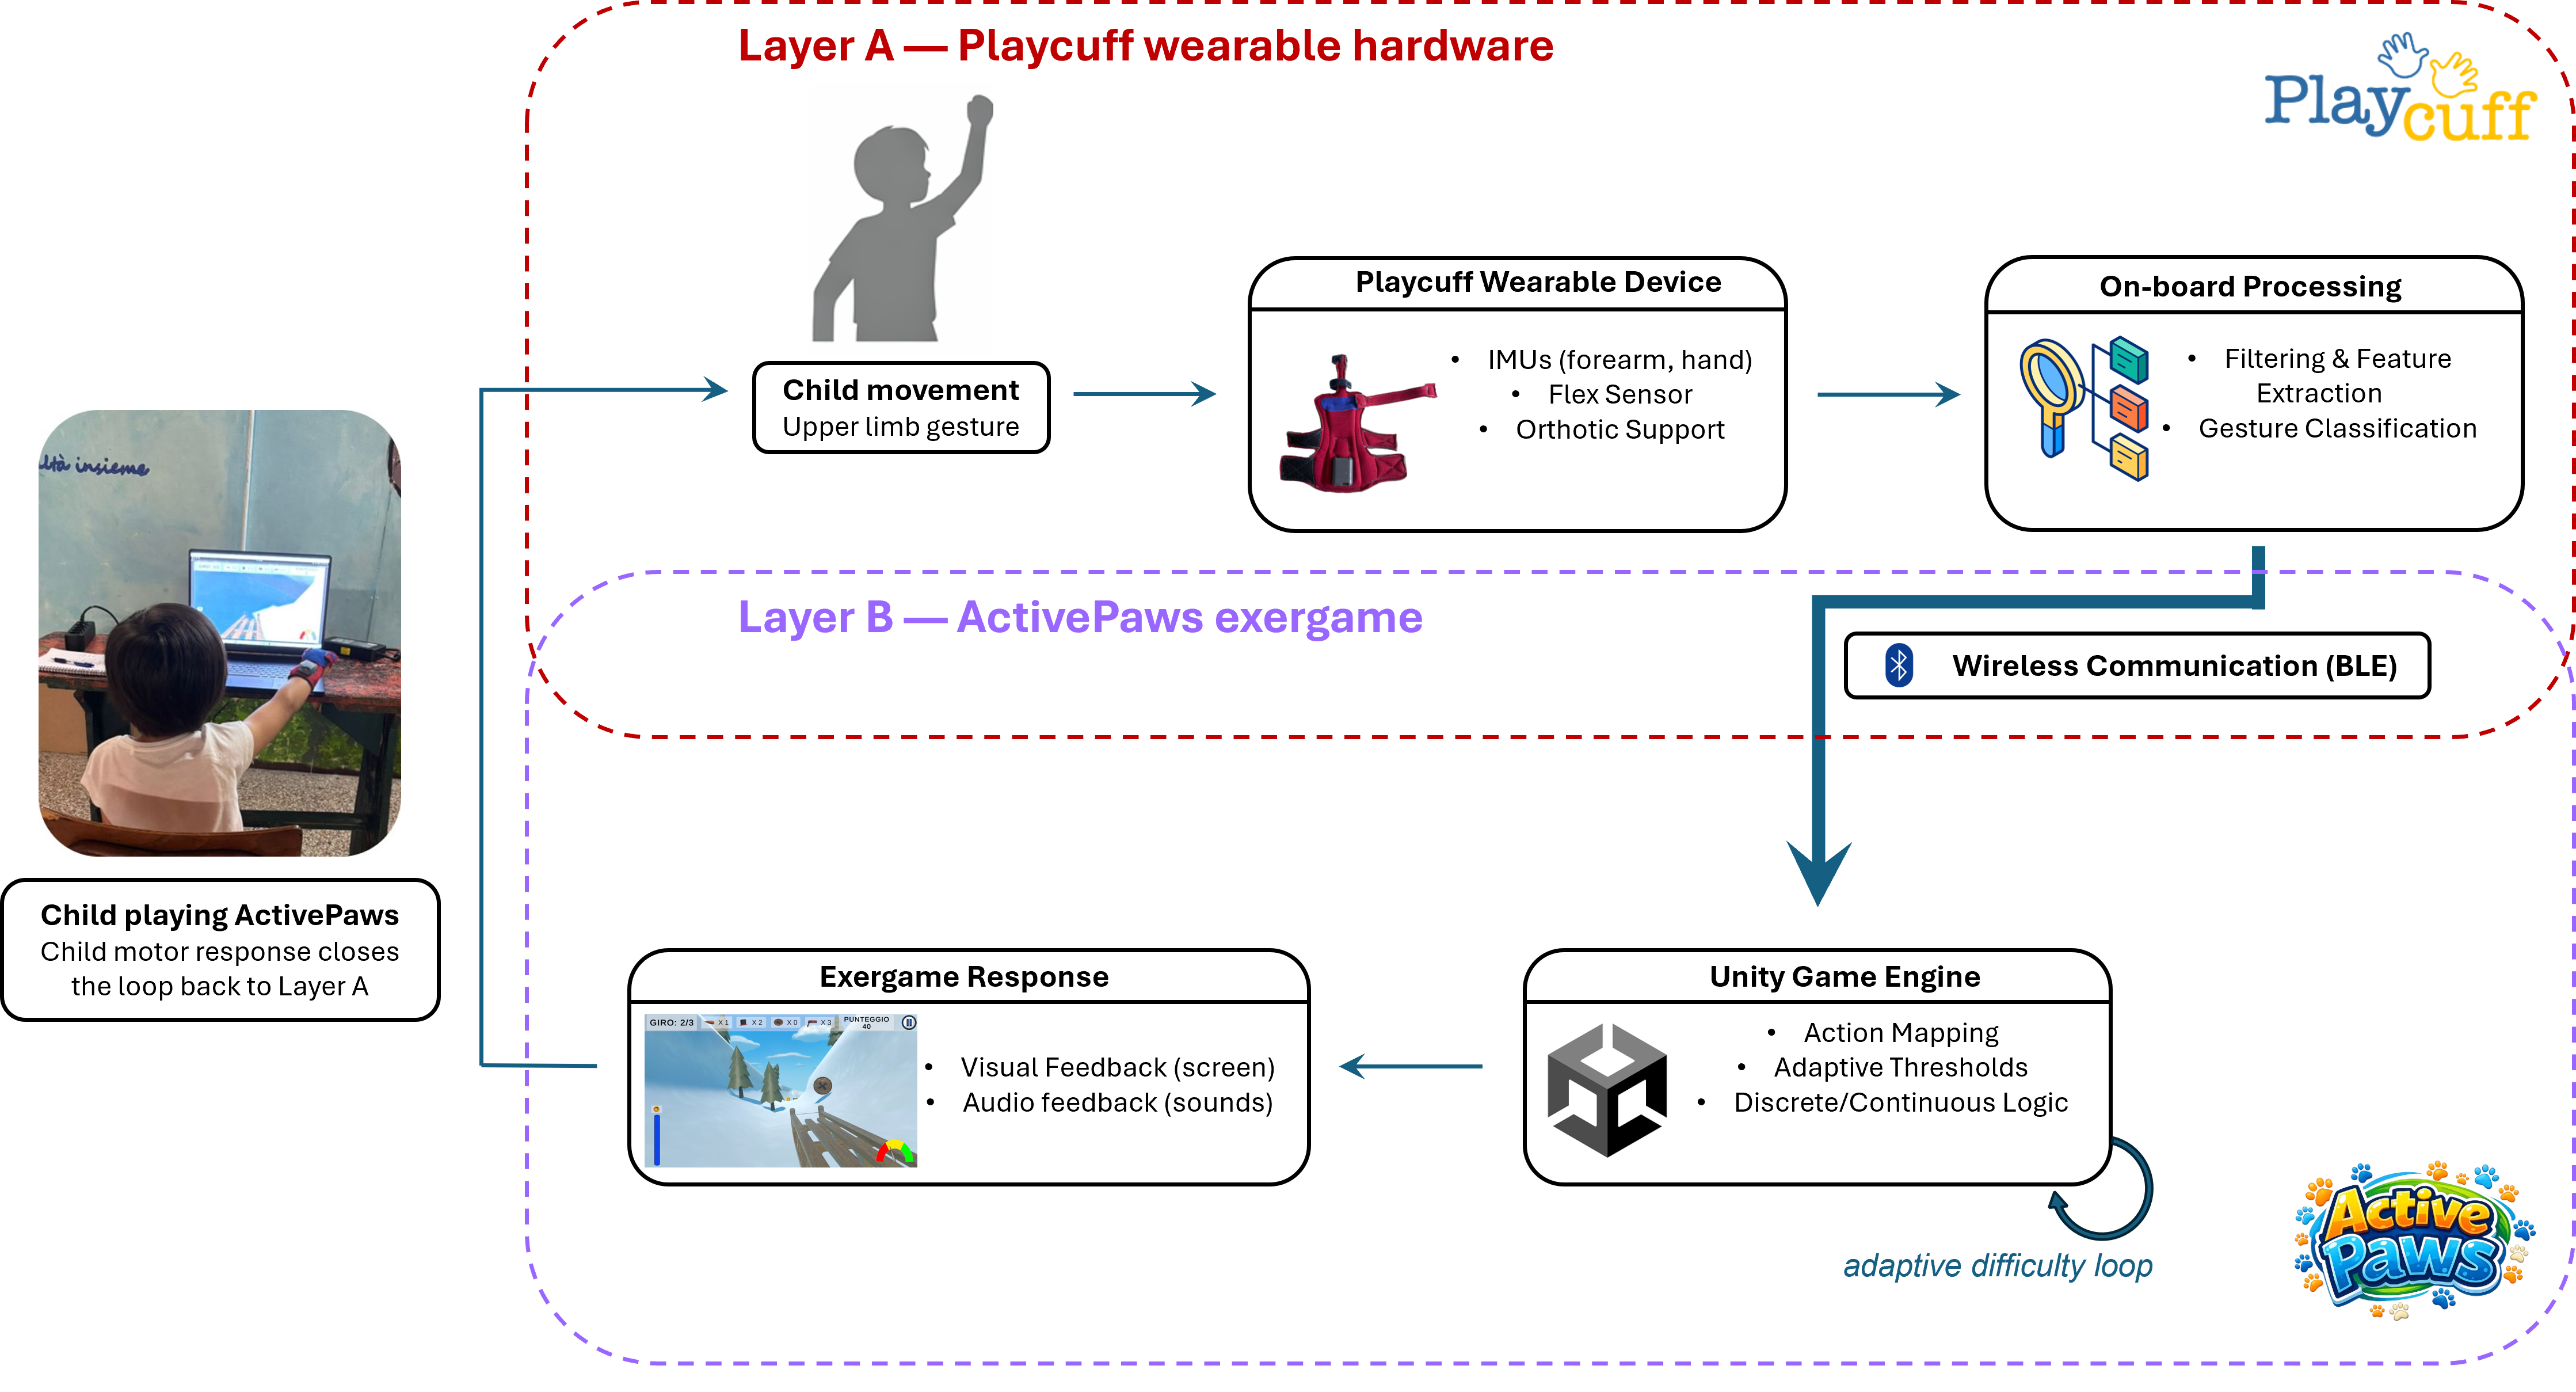
\includegraphics[width=\columnwidth]{figures/AP/AP_Scheme.png}
	
	\small Layer A: Playcuff orthosis with sensing. Layer B: Unity exergame suite with game logic and personalization. Layer C: Therapist configuration interface for clinical customization.
\end{frame}

\begin{frame}{Playcuff Wristband: Form Factor and Orthotic Function}
	\textbf{\textcolor{gbAqua}{Physical Design}}
	
	\begin{itemize}
		\item Soft neoprene wristband (midway between band and glove)
		\item Multiple adjustable sizes for different age groups
		\item Worn via Velcro straps: NO gripping effort required
		\item Designed for children with variable motor abilities
	\end{itemize}
	
	\vspace{0.3cm}
	
	\textbf{\textcolor{gbAqua}{Why ``Worn'' Not ``Held'' Matters}}
	
	\begin{itemize}
		\item Traditional controllers demand sustained grip, precise finger coordination
		\item Playcuff frees hand for natural movement
		\item Supports seated, standing, or mobile play
	\end{itemize}
	
	\vspace{0.3cm}
	
	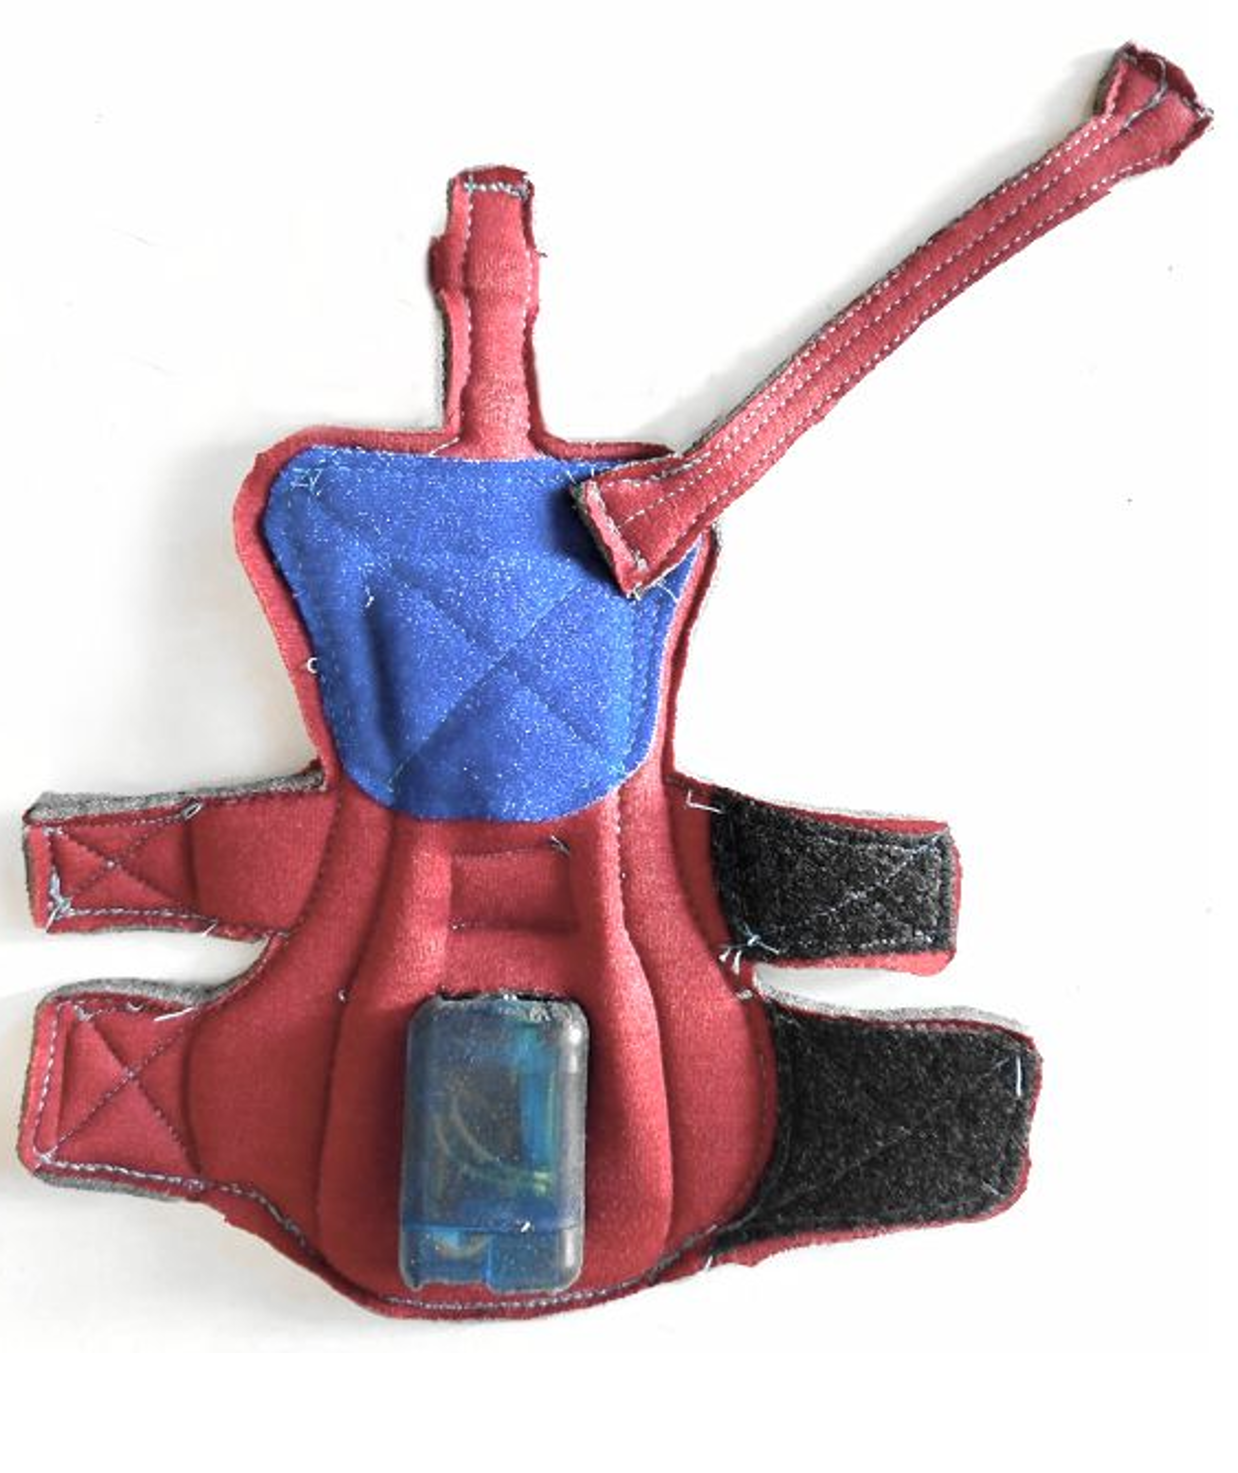
\includegraphics[width=0.8\columnwidth]{figures/AP/Playcuff.png}
	
	\citefooter{Lazzari et al., 2026}
\end{frame}

\begin{frame}{Playcuff: Sensing and Gesture Classification}
	\textbf{\textcolor{gbAqua}{Orthotic Function: NiTi Splints}}
	
	\begin{itemize}
		\item Nickel-Titanium pseudoelastic bars in curved channels
		\item Provide mild restoring force toward neutral position
		\item Resist sudden movements (absorb tremor energy)
		\item Enhance proprioceptive feedback for better motor control
	\end{itemize}
	
	\vspace{0.3cm}
	
	\textbf{\textcolor{gbAqua}{Sensing Suite}}
	
	\begin{itemize}
		\item 2× IMU (forearm + hand): accelerometer, gyroscope, magnetometer
		\item 1× Flex sensor: metacarpophalangeal joint flexion
		\item 200 Hz acquisition, 40 Hz preprocessing on-board MCU
	\end{itemize}
	
	\vspace{0.3cm}
	
	\textbf{\textcolor{gbAqua}{Two-Tiered Classification}}
	
	\begin{itemize}
		\item Tier 1 (Forearm): 6 features → 18 classes (94% accuracy)
		\item Tier 2 (Wrist): 5 features → 4 classes (99.5% accuracy)
		\item Speed levels: Slow / Medium / High
		\item Total: 33 distinct gesture classes
	\end{itemize}
	
	\citefooter{Lazzari et al., 2026}
\end{frame}

\begin{frame}{Playcuff: Wireless Control and Immediate Usability}
	\textbf{\textcolor{gbAqua}{Gesture Transmission}}
	
	\begin{itemize}
		\item Wireless Bluetooth at 40 Hz
		\item Compact packets: forearm class, wrist class, hand state, speed
		\item Sliding time window acceptance: filters spurious classifications
		\item Makes interaction robust even with irregular movements
	\end{itemize}
	
	\vspace{0.3cm}
	
	\textbf{\textcolor{gbAqua}{Discrete vs Continuous Actions}}
	
	\begin{columns}[t]
		\column{0.48\textwidth}
		\textbf{Discrete} (e.g., shooting)
		
		\begin{itemize}
			\item Accept on detection
			\item Refractory period prevents unintended repetition
		\end{itemize}
		
		\column{0.48\textwidth}
		\textbf{Continuous} (e.g., steering)
		
		\begin{itemize}
			\item Speed-dependent displacement
			\item Effort-to-effect mapping
		\end{itemize}
	\end{columns}
	
	\vspace{0.3cm}
	
	\textbf{\textcolor{gbAqua}{CRITICAL FEATURE: NO Calibration}}
	
	Device ready immediately upon connection—no setup steps required (essential for children and clinical settings)
\end{frame}

\begin{frame}{Swift Rescuer Game: Protecting Animals}
	\textbf{\textcolor{gbAqua}{Gameplay Concept}}
	
	Protect animals from incoming obstacles by aiming and shooting
	
	\vspace{0.2cm}
	
	\textbf{\textcolor{gbAqua}{Therapeutic Goals}}
	
	\begin{itemize}
		\item Wrist extension for aiming
		\item Rapid wrist flexion for shooting
		\item Sustained forearm positioning
		\item Eye-hand coordination and precision
	\end{itemize}
	
	\vspace{0.2cm}
	
	\textbf{\textcolor{gbAqua}{Game Mechanics}}
	
	\begin{itemize}
		\item Gesture mapping: Wrist rotation → crosshair movement
		\item Action: Wrist flexion → shoot projectile
		\item Target: Hit moving animals, protect from obstacles
		\item Progression: Three difficulty levels with increased speed and obstacles
	\end{itemize}
	
	\vspace{0.2cm}
	
	\textbf{\textcolor{gbAqua}{Design Features}}
	
	Alternative movements for diverse abilities; semantically coherent gestures; immediate visual/audio feedback; thematically coherent environment
\end{frame}

\begin{frame}{Sledding Adventures Game: Dynamic Navigation}
	\textbf{\textcolor{gbAqua}{Gameplay Concept}}
	
	Navigate sledding character down slopes, avoiding obstacles, collecting coins
	
	\vspace{0.2cm}
	
	\textbf{\textcolor{gbAqua}{Therapeutic Goals}}
	
	\begin{itemize}
		\item Forearm rotation for steering (pronation/supination)
		\item Arm lifting for jumping
		\item Whole-arm coordination
		\item Dynamic balance and movement control
	\end{itemize}
	
	\vspace{0.2cm}
	
	\textbf{\textcolor{gbAqua}{Game Mechanics}}
	
	\begin{itemize}
		\item Gesture mapping: Forearm rotation → sled steering left/right
		\item Action: Arm lift → sled jump over obstacles
		\item Reward: Collect coins, maintain momentum
		\item Progression: Faster slopes, tighter turns, more obstacles
	\end{itemize}
	
	\vspace{0.2cm}
	
	\textbf{\textcolor{gbAqua}{Design Features}}
	
	Semantic coherence (rotate to follow curves); smooth immediate feedback; three progressively challenging levels
\end{frame}

\begin{frame}{Galaxy Drift Game: Precision Control}
	\textbf{\textcolor{gbAqua}{Gameplay Concept}}
	
	Control spacecraft through asteroid fields, collect crystals, achieve high scores
	
	\vspace{0.2cm}
	
	\textbf{\textcolor{gbAqua}{Therapeutic Goals}}
	
	\begin{itemize}
		\item Fine wrist control and precision
		\item Sustained attention and planning
		\item Speed vs accuracy trade-off
		\item Rapid response to changing environments
	\end{itemize}
	
	\vspace{0.2cm}
	
	\textbf{\textcolor{gbAqua}{Game Mechanics}}
	
	\begin{itemize}
		\item Gesture mapping: Wrist flexion/extension → vertical movement
		\item Action: Forearm rotation → horizontal displacement
		\item Objective: Avoid asteroids, collect crystals
		\item Progression: Score-based with leaderboard
	\end{itemize}
	
	\vspace{0.2cm}
	
	\textbf{\textcolor{gbAqua}{Design Features}}
	
	Combines precision and speed; engaging space theme; dynamic music; real-time score feedback; adaptive difficulty scaling
\end{frame}

\begin{frame}{Design Philosophy: Semantic Coherence and Accessibility}
	\textbf{\textcolor{gbAqua}{Semantic Coherence}}
	
	\begin{itemize}
		\item Movement mapping intuitive and related to effect
		\item Rotate wrist to aim, lift arm to jump, twist to steer
		\item Reduces cognitive load, enables intuitive learning
	\end{itemize}
	
	\vspace{0.2cm}
	
	\textbf{\textcolor{gbAqua}{Accessibility: Alternative Gestures}}
	
	\begin{itemize}
		\item Multiple ways to achieve same in-game action
		\item Accommodates heterogeneous impairment profiles
		\item Ensures no child excluded from any game aspect
	\end{itemize}
	
	\vspace{0.2cm}
	
	\textbf{\textcolor{gbAqua}{Visual Clarity}}
	
	\begin{itemize}
		\item Rich enough to engage (commercial-game appearance)
		\item Uncluttered enough to reduce cognitive overload
		\item Thematic coherence aids narrative immersion
	\end{itemize}
	
	\vspace{0.2cm}
	
	\textbf{\textcolor{gbAqua}{Multimodal Feedback}}
	
	Visual + Audio + Haptic cues reinforce successful execution and maintain engagement across sessions
\end{frame}

\begin{frame}{Therapist Interface: Personalization for Clinical Use}
	\textbf{\textcolor{gbAqua}{Configurability Dimensions}}
	
	\begin{columns}[t]
		\column{0.48\textwidth}
		\textbf{Movement Mapping}
		
		\begin{itemize}
			\item Remap gestures to actions
			\item Adjust intensity thresholds
			\item Enable/disable alternative movements
		\end{itemize}
		
		\column{0.48\textwidth}
		\textbf{Game Parameters}
		
		\begin{itemize}
			\item Target speed and frequency
			\item Difficulty progression
			\item Session duration
			\item Reward magnitude
		\end{itemize}
	\end{columns}
	
	\vspace{0.3cm}
	
	\textbf{\textcolor{gbAqua}{Adaptive Features}}
	
	\begin{itemize}
		\item Real-time performance monitoring
		\item Automatic difficulty adjustment
		\item Gesture calibration phase to compensate for sensor drift
		\item Personalized movement ranges and intensity
	\end{itemize}
	
	\vspace{0.2cm}
	
	\textit{Core principle: Clinical expertise shapes design; implementation outcomes feed back into clinical expectations}
\end{frame}

\begin{frame}{Pilot Evaluation: Study Design and Protocol}
	\textbf{\textcolor{gbAqua}{Participants}}
	
	\begin{itemize}
		\item 11 typically developing children (age 6-14, median 9.5)
		\item Recruited from summer camps
		\item Most familiar with video games
		\item Preliminary step before clinical trials with neuromotor disorders
	\end{itemize}
	
	\vspace{0.3cm}
	
	\textbf{\textcolor{gbAqua}{Protocol}}
	
	\begin{itemize}
		\item Session duration: ~20 minutes
		\item Three phases: Donning Playcuff → Gameplay → Post-game questionnaire
		\item Tablet-based questionnaire with emoji scales (kid-friendly)
		\item Adults present for comprehension support
	\end{itemize}
	
	\vspace{0.3cm}
	
	\textbf{\textcolor{gbAqua}{Measurements}}
	
	\begin{itemize}
		\item Subjective: Enjoyment, Usability (SUS for Kids), Engagement (UES-SF)
		\item Objective: Game logs (accuracy, progression), movement tracking
	\end{itemize}
	
	\citefooter{Pizzo et al., ``ActivePaws and Playcuff: Pilot Evaluation of Non-Immersive Exergame Suite,'' IEEE ISMAR-Adjunct, 2025}
\end{frame}

\begin{frame}{Pilot Evaluation: Engagement and Usability Results}
	\textbf{\textcolor{gbAqua}{Enjoyment: 100\% Positive}}
	
	\begin{itemize}
		\item 100\% found games fun
		\item 91\% would play again (1 said ``Maybe'')
		\item 8/11 preferred Sledding Adventures over Swift Rescuer
		\item 100\% reported feeling good or proud while playing
	\end{itemize}
	
	\vspace{0.3cm}
	
	\textbf{\textcolor{gbAqua}{Usability: High Accessibility}}
	
	\begin{itemize}
		\item 80\%+ no confusion about controls
		\item 80\%+ found games easy to use
		\item 90\%+ no anger/annoyance during play
		\item 80\%+ believed friends would quickly learn
	\end{itemize}
	
	\vspace{0.3cm}
	
	\textbf{\textcolor{gbAqua}{Engagement: Sustained Attention}}
	
	\begin{itemize}
		\item 45\% felt ``very absorbed'' (forgot everything)
		\item 36\% felt ``somewhat'' absorbed
		\item 100\% appreciated colors and graphics
		\item 100\% found activity fun and enjoyable
	\end{itemize}
	
	\vspace{0.2cm}
	
	\alert{RQ4 Answer: YES – ActivePaws achieves high engagement and usability}
	
	\citefooter{Pizzo et al., 2025}
\end{frame}

%% ══════════════════════════════════════════════════════════════════════════════
%% PART 8: CONCLUSIONS (3 SLIDES)
%% ══════════════════════════════════════════════════════════════════════════════

\begin{frame}{Research Questions Answered}
	\textbf{\textcolor{gbAqua}{RQ1: Which 3D reconstruction software for non-experts?}}
	
	\alert{Answer:} 3DF Zephyr best trade-off. Colmap for accuracy-critical applications.
	
	\vspace{0.2cm}
	
	\textbf{\textcolor{gbAqua}{RQ2: Are off-the-shelf reconstructions good enough?}}
	
	\alert{Answer:} YES – Kinect v1, ReCap Photo, photogrammetry produce functionally sufficient reconstructions for XR.
	
	\vspace{0.2cm}
	
	\textbf{\textcolor{gbAqua}{RQ3: Which non-immersive modality best approximates IVR?}}
	
	\alert{Answer:} Fixed perspective projection optimal. Orthographic viable alternative. Tracked perspective NOT recommended.
	
	\vspace{0.2cm}
	
	\textbf{\textcolor{gbAqua}{RQ4: Can wearable-controlled exergame achieve engagement?}}
	
	\alert{Answer:} YES – ActivePaws demonstrates high engagement (100\% fun), usability (80\%+ accessibility), effective movement-to-gameplay translation.
\end{frame}

\begin{frame}{Overall Contributions: Complementary Dimensions}
	\textbf{\textcolor{gbAqua}{Safety through Spatial Coherence}}
	
	\begin{itemize}
		\item 3D reconstruction achievable without prohibitive cost or expertise
		\item Functional evaluation more relevant than geometric benchmarking
		\item Democratizes XR for training and simulation
	\end{itemize}
	
	\vspace{0.3cm}
	
	\textbf{\textcolor{gbAqua}{User Experience through Evidence-Based Design}}
	
	\begin{itemize}
		\item Clinical constraints require non-immersive modalities
		\item Visualization selection must be empirically informed
		\item Fixed perspective optimal non-immersive choice for rehabilitation
	\end{itemize}
	
	\vspace{0.3cm}
	
	\textbf{\textcolor{gbAqua}{Engagement through Co-Design}}
	
	\begin{itemize}
		\item Wearable-based interaction accommodates heterogeneous abilities
		\item Semantic coherence enhances intuitiveness
		\item Therapist collaboration ensures clinical relevance alongside engagement
		\item Movement-based interaction effectively translates to meaningful gameplay
	\end{itemize}
	
	\vspace{0.2cm}
	
	\alert{Synthesis:} Three dimensions complementary; together enable XR systems simultaneously safe, accessible, engaging, and therapeutically effective
\end{frame}

\begin{frame}{Limitations and Future Work}
	\textbf{\textcolor{gbAqua}{Limitations}}
	
	\begin{itemize}
		\item Studies 1-2: Limited to indoor rooms and photogrammetry; generalizability uncertain
		\item Study 3: Healthy adults; may not generalize to clinical population
		\item ActivePaws: Pilot with typically developing children; clinical efficacy not yet demonstrated
	\end{itemize}
	
	\vspace{0.3cm}
	
	\textbf{\textcolor{gbAqua}{Clinical Translation Path}}
	
	\begin{itemize}
		\item ActivePaws longitudinal study with children with cerebral palsy
		\item Assess therapeutic outcomes: motor learning, engagement over time
		\item Evaluate adaptive features and therapist personalization effectiveness
		\item Fit4MedRob project collaboration ongoing
	\end{itemize}
	
	\vspace{0.3cm}
	
	\textbf{\textcolor{gbAqua}{Broader XR Implications}}
	
	\begin{itemize}
		\item Extend visualization guidance to other clinical contexts
		\item Develop open-source 3D reconstruction workflows
		\item Establish best practices for therapist-developer collaboration
		\item Contribute to XR evaluation methodologies standardization
	\end{itemize}
\end{frame}